\documentclass{article}
\usepackage{tikz,amsmath,tkz-graph,caption,float}
\usetikzlibrary{shapes,arrows,fit,calc,positioning,decorations.pathreplacing}
\tikzset{box/.style={draw, thick, text centered, minimum height=0.5cm, minimum width=1cm}}
\tikzset{line/.style={draw, thick, -latex'}}
\title{CSC 226 Problem Set 1 Written Part}
\author{%
	Oliver Tonnesen\\
	V00885732}
\date{September 29, 2018}
\begin{document}
\maketitle
\section{Lower bounds for sorting}
	We define $S_m$ to be the sequence $\{x_{(m-1)k+1},x_{(m-1)k+2}\ldots{x_{mk}}\}$.\\
	\newline
	\newline
	\newline
	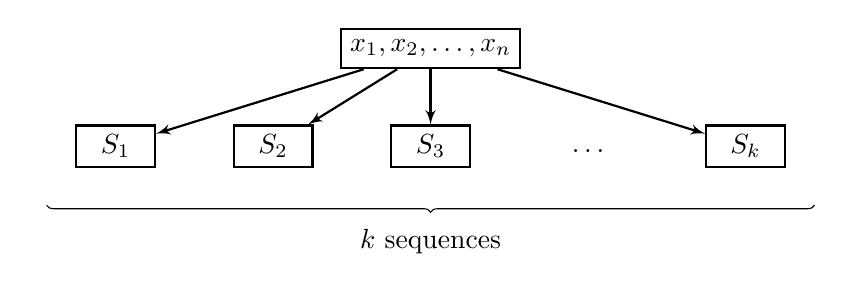
\begin{tikzpicture}
		\node [box]										(1) {${x_1,x_2,\ldots,x_n}$};
		\node [box, below=0.7cm of 1, xshift=-4cm]		(2) {$S_1$};
		\node [box, below=0.7cm of 1, xshift=-2cm]		(3) {$S_2$};
		\node [box, below=0.7cm of 1, xshift=0cm]		(4) {$S_3$};
		\node [below=0.9cm of 1, xshift=2cm]			(5) {$\ldots$};
		\node [box, below=0.7cm of 1, xshift=4cm]		(6) {$S_k$};
		\node [below=0.9cm of 1, xshift=-5cm]			(L) {};
		\node [below=0.9cm of 1, xshift=5cm]			(R) {};

		\path [line] (1) -> (2);
		\path [line] (1) -> (3);
		\path [line] (1) -> (4);
		% \path [line] (1) -> (5);
		\path [line] (1) -> (6);

		\draw [decoration={brace,mirror,raise=20pt}, decorate] (L) -- node [style={below=25pt}, pos=0.5] {$k$ sequences} (R);
	\end{tikzpicture}
	\newline
	\newline
	\newline
	Since each sequence is of length $k$, each can be sorted in $\Omega(k\log{k})$ comparisons. $k$ sequences need to be sorted,
	so sorting the entire sequence takes $\Omega(k^2\log{k})$ comparisons. Note that $k^2=n$, so $\Omega(k^2\log{k})$ is equivalent
	to ${\Omega(n\log{k})}$, and so the entire sequence can therefore be sorted in $\Omega(n\log{k})$ time.
\section{Quickselect with median-of-medians pivots}
	For each iteration of select finding the median of medians, at least half of the medians are $\ge$ the actual median of medians.
	So at least half of the $~\frac{n}{9}$ groups contribute $\ge5$ elements that are greater than the median of medians (assuming distinct elements).
	\[5\cdot\frac{1}{2}\cdot\frac{n}{9}=\frac{5n}{18}\]
	So at least $\frac{5n}{18}$ elements are greater than the median of medians. Conversely, at most $\frac{13n}{18}$ elements are lesser than the
	median of medians, and likewise at most $\frac{13n}{18}$ elements are greater than the median of medians. So we can set up our recurrence as follows:
	\[T(n)=T{\bigg(\frac{13n}{18}\bigg)}+T{\bigg(\frac{n}{9}\bigg)}+cn\]
	\begin{tikzpicture}[every node/.style={minimum size=.5cm-\pgflinewidth, outer sep=0pt}]
		\node [below=0.9cm of 1,xshift=10cm,yshift=2cm]			(top) {};
		\node [below=0.9cm of 1,xshift=10cm,yshift=-5cm]			(bottom) {};
		\draw [decoration={brace,raise=20pt}, decorate] (top) -- node [style={right=25pt}, pos=0.5] {$\infty$} (bottom);

		\filldraw[draw=black,fill=white] (0,0) rectangle (9,-1) node[pos=.5] {$cn$};
		\filldraw[draw=black,fill=white] (0,-1) rectangle (7,-2) node[pos=.5] {$\frac{7cn}{9}$};
		\filldraw[draw=black,fill=white] (7,-1) rectangle (8,-2) node[pos=.5] {$\frac{cn}{9}$};
		\filldraw[draw=black,fill=white] (0,-2) rectangle (5.44,-3) node[pos=.5] {$\frac{7cn}{9}$};
		\filldraw[draw=black,fill=white] (5.44,-2) rectangle (6.22,-3) node[pos=.5] {$\frac{7cn}{81}$};
		\filldraw[draw=black,fill=white] (6.22,-2) rectangle (7,-3) node[pos=.5] {$\frac{7cn}{81}$};
		\filldraw[draw=black,fill=white] (7,-2) rectangle (7.11,-3) node[pos=.5,yshift=-10mm] {$\frac{cn}{81}$};
		\filldraw[draw=white,fill=white] (0,-3.01) rectangle (9,-5) node[pos=.5] {\vdots};
		\filldraw[draw=black,fill=white] (3.5,-5.01) rectangle (5.5,-6) node[pos=.5] {Base Case};
	\end{tikzpicture}
	\newline
	\begin{align*}
		&=\sum_{i=0}^{\infty}cn{\bigg(\frac{15}{18}\bigg)}^i\\
		&=\frac{cn}{1-\frac{15}{18}}\\
		&=6cn\\
		&\in{O(n)}
	\end{align*}
\section{Insertion in 2\--3 trees}
\captionsetup[figure]{labelformat=empty}
	\begin{figure}[H]
		\centering
		\begin{minipage}{.33\textwidth}
			\centering
			\documentclass[11pt]{article}
\usepackage{fancyhdr}
\pagestyle{fancy}
\newcommand\course{MATH 423}
\newcommand\hwnumber{1}
\newcommand\duedate{September 26, 2019}

\lhead{Oliver Tonnesen\\V00885732}
\chead{\textbf{\Large Project \hwnumber}}
\rhead{\course\\\duedate}


\usepackage{cite}
\usepackage{url}


\usepackage{tikz}


\usepackage{float}


\usepackage{amsmath,amsfonts,amsthm}


\begin{document}


\section{Introduction}
\subsection{Background}
The minimum-weight spanning tree problem is one of the oldest studied problems
in graph theory. Given a connected, edge-weighted graph, a minimum-weight
spanning tree is a subgraph that is connected, acyclic, and whose edge weights
sum to the minimum possible value.

The first published solution to the minimum-weight spanning tree problem is due
to Bor\r{u}vka in 1926\cite{Boruvka}. In his paper, Bor\r{u}vka devotes a section to the
application of his method to the design of electricity power networks. The
example he uses is his home region of Moravia.

The single-source shortest path problem is a more recent problem. Given a
connected, edge-weighted graph, and a vertex $s$ in it, a correct solution is a
subgraph that is connected, acyclic, and in which any path from $s$ to any
other vertex has minimal weight.

This paper aims to briefly survey some of the classical methods of solving the
above problems. Specifically, we investigate Kruskal and Prim's algorithms, two
methods of solving the minimum-weight spanning tree problem, and Dijkstra's
algorithm, a method of solving a special case of the single-source shortest
path problem where the given graph has only nonnegative edge weights.


\subsection{Applications}
There are many useful applications of minimum-weight spanning trees. Some of
their most obvious applications are those for which they were originally
studied: physical networks, such as electrical networks, transportation systems,
water networks, computer and telecommunications networks, among others. Some
less obvious applications include optimally broadcasting information throughout
all computers in a connected network, circuit design, or finding paths in a
system with maximum bottleneck.

Some applications of solving the single-cource shortest path problem are
finding optimal paths for GPS navigation, routing in telecommunications
networks, or updating computers in a network from a central server.


\subsection{Definitions}
We define some terms we will use in this paper:
\newline
\newline
\textbf{\underline{MST}}: Given a connected, undirected graph $G=(V(G),E(G))$,
with weight function $w:E(G)\rightarrow\mathbb{R}$, a MST of $G$ is a connected,
acyclic subgraph $T=(V(G),E(T))$ such that $\Sigma_{e\in E(T)}w(e)$ is minimal.
\newline
\newline
\textbf{\underline{Cut}}: Given a graph $G=(V(G),E(G))$ and a subset
$S\subseteq V(G)$, a cut $(S,V(G)\setminus S)$ of $G$ is a partition of $V$.
An edge $e\in E(G)$ \textbf{\underline{crosses}} $(S,V(G)\setminus S)$ if $e$
has one endpoint in either partition of the cut. A cut
\textbf{\underline{respects}} a set $A$ of edges if no edge in $A$ crosses the
cut.
\newline
\newline
\textbf{\underline{Light edge}}: An edge is called \underline{light} for a cut
$(S,V(G)\setminus S)$ if it is a minimal weight edge crossing it.
\newline
\newline
\textbf{\underline{Safe edge}}: Let $A\subseteq E$ be a subset of a MST. An
edge $e\in E$ is called \underline{safe} for $A$ if $A\cup\{e\}$ is still a
subset of a MST.
\newline
\newline
\textbf{\underline{Path weight}}: If $P$ is a path with edges $e_1,\ldots,e_k$,
then define the weight of $P$, $w(P)$ as $\sum_{i=1}^kw(e_i)$.
\newline
\newline
\textbf{\underline{Minimal path}}: Let $G=(V(G),E(G))$ and $u,v\in V(G)$. Then
define $\delta(u,v)=\min\{w(P)\mid\text{$P$ is a $u,v$-path in $G$}\}$.


\subsection{Examples}

\begin{figure}[H]
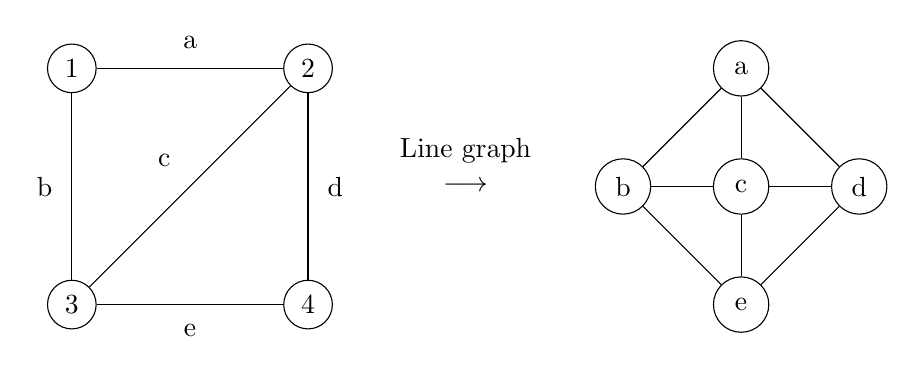
\begin{tikzpicture}[black/.style={circle,draw,fill=black,inner sep=0pt, minimum width=4pt}]
\node[circle,draw] at (0,3) (1) {1};
\node[circle,draw] at (3,3) (2) {2};
\node[circle,draw] at (0,0) (3) {3};
\node[circle,draw] at (3,0) (4) {4};

\draw (1) -- (2) node [midway,label=above:{a}] {};
\draw (1) -- (3) node [midway,label=left:{b}] {};
\draw (2) -- (3) node [midway,label=above left:{c}] {};
\draw (2) -- (4) node [midway,label=right:{d}] {};
\draw (3) -- (4) node [midway,label=below:{e}] {};


\draw node at (5, 1.5) {$\longrightarrow$};
\draw[above,yshift=5] node at (5,1.5) {Line graph};


\node[circle,draw,minimum width=20pt] at (8.5,3) (a) {a};
\node[circle,draw,minimum width=20pt] at (7,1.5) (b) {b};
\node[circle,draw,minimum width=20pt] at (8.5,1.5) (c) {c};
\node[circle,draw,minimum width=20pt] at (10,1.5) (d) {d};
\node[circle,draw,minimum width=20pt] at (8.5,0) (e) {e};

\draw (a) -- (b);
\draw (a) -- (c);
\draw (a) -- (d);
\draw (b) -- (c);
\draw (b) -- (e);
\draw (c) -- (d);
\draw (c) -- (e);
\draw (d) -- (e);
\end{tikzpicture}

\end{figure}
\begin{figure}[H]
\begin{tikzpicture}[black/.style={circle,draw,fill=black,inner sep=0pt,minimum width=4pt}]
\node[black] at (0,0) (0) {};
\foreach \number in {1,...,8}
{
	\mycount=\number
	\advance\mycount by -1
	\multiply\mycount by 45
	\advance\mycount by 0
	\node[black] (\number) at (\the\mycount:1cm) {};
	\draw (0) -- (\number);
}


\draw node at (3, 0) {$\longrightarrow$};
\draw[above,yshift=5] node at (3,0) {Line graph};


\foreach \number in {1,...,8}
{
	\mycount=\number
	\advance\mycount by -1
	\multiply\mycount by 45
	\advance\mycount by 0
	\node[black,xshift=160] (\number) at (\the\mycount:1cm) {};
}
\foreach \x in {1,...,8}
	\foreach \y in {\x,...,8}
		\draw (\x) -- (\y);


\end{tikzpicture}

\end{figure}
\begin{figure}[H]
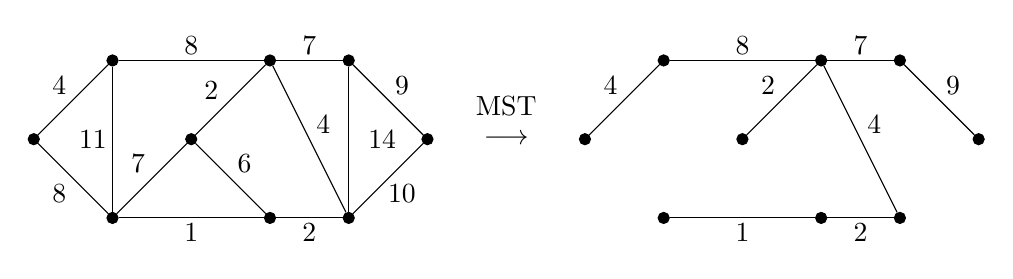
\begin{tikzpicture}[black/.style={circle,draw,fill=black,inner sep=0pt, minimum width=4pt}]
	\foreach \x in {1,3,4}
		\node[black] at (\x,2) (a\x) {};
	\foreach \x in {0,2,5}
		\node[black] at (\x,1) (b\x) {};
	\foreach \x in {1,3,4}
		\node[black] at (\x,0) (c\x) {};
	\draw (a1) -- (a3) node [midway,label={8},yshift=-5] {};
	\draw (a3) -- (a4) node [midway,label={7},yshift=-5] {};
	\draw (c1) -- (c3) node [midway,label=below:{1},yshift=5] {};
	\draw (c3) -- (c4) node [midway,label=below:{2},yshift=5] {};
	\draw (b0) -- (a1) node [midway,label={4},xshift=-5,yshift=-5] {};
	\draw (b0) -- (c1) node [midway,label=below:{8},xshift=-5,yshift=5] {};
	\draw (a1) -- (c1) node [midway,label=left:{11},xshift=5] {};
	\draw (c1) -- (b2) node [midway,label={7},xshift=-5,yshift=-5] {};
	\draw (b2) -- (c3) node [midway,label={6},xshift=5,yshift=-5] {};
	\draw (b2) -- (a3) node [midway,label={2},xshift=-7,yshift=-7] {};
	\draw (a3) -- (c4) node [midway,label={4},xshift=5,yshift=-5] {};
	\draw (a4) -- (b5) node [midway,label={9},xshift=5,yshift=-5] {};
	\draw (c4) -- (b5) node [midway,label=below:{10},xshift=5,yshift=5] {};
	\draw (a4) -- (c4) node [midway,label=right:{14}] {};


	\draw node at (6,1) {$\longrightarrow$};
	\draw[above,yshift=5] node at (6,1) {MST};


	\foreach \x in {8,10,11}
		\node[black] at (\x,2) (aa\x) {};
	\foreach \x in {7,9,12}
		\node[black] at (\x,1) (bb\x) {};
	\foreach \x in {8,10,11}
		\node[black] at (\x,0) (cc\x) {};
	\draw (aa8) -- (aa10) node [midway,label={8},yshift=-5] {};
	\draw (aa10) -- (aa11) node [midway,label={7},yshift=-5] {};
	\draw (cc8) -- (cc10) node [midway,label=below:{1},yshift=5] {};
	\draw (cc10) -- (cc11) node [midway,label=below:{2},yshift=5] {};
	\draw (bb7) -- (aa8) node [midway,label={4},xshift=-5,yshift=-5] {};
	% \draw (bb7) -- (cc8) node [midway,label=below:{8},xshift=-5,yshift=5] {};
	% \draw (aa8) -- (cc8) node [midway,label=left:{11},xshift=5] {};
	% \draw (cc8) -- (bb9) node [midway,label={7},xshift=-5,yshift=-5] {};
	% \draw (bb9) -- (cc10) node [midway,label={6},xshift=5,yshift=-5] {};
	\draw (bb9) -- (aa10) node [midway,label={2},xshift=-5,yshift=-5] {};
	\draw (aa10) -- (cc11) node [midway,label={4},xshift=5,yshift=-5] {};
	\draw (aa11) -- (bb12) node [midway,label={9},xshift=5,yshift=-5] {};
	% \draw (cc11) -- (bb12) node [midway,label=below:{10},xshift=5,yshift=5] {};
	% \draw (aa11) -- (cc11) node [midway,label=right:{14}] {};
\end{tikzpicture}

\end{figure}

\section{Algorithms for finding minimum spanning trees}


\subsection{A generic MST algorithm}
The two algorithms we consider in this paper both share very similar structure.
The following generic MST algorithm will form the basis for both Kruskal and
Prim's algorithms:
\newline
Given $G=(V(G),E(G))$. Start with the $T=\emptyset$. This will form a subset of
$E(G)$ that will induce a MST of $G$. Apply the following step until
$V(G[T])=V(G)$: pick an edge $e$ that is safe for $T$, and let $T=T\cup\{e\}$.
\cite{CLRS}

We first prove the correctness of this algorithm, then use its correctness to
more easily prove the correctness of Kruskal and Prim's algorithms.
\begin{proof}
	We wish to show that at the termination of this algorithm, $G[T]$ is a
	MST. Every edge added to $T$ is safe, so whenever
	an edge is added to $T$, $G[T]$ remains a subgraph of some minimum-weight
	spanning tree. Thus after adding $n(G)-1$ edges to $T$, $G[T]$ is still a
	subgraph of a MST. But any tree has only $n(G)-1$
	edges, so $G[T]$ is a MST.
\end{proof}


\subsection{Kruskal's algorithm}
Given $G=(V(G),E(G))$. First the edges are sorted into a list in order of
nondecreasing weight. Start with $T=\emptyset$. Apply the following step until
$n(G)-1$ edges have been chosen: if the lowest weight edge $e$ has both
endpoints in the same component of $G[T]$, ignore it. Otherwise, let
$T=T\cup\{e\}$. Remove $e$ from the list.\cite{MST}


\subsection{Examples}
\begin{figure}[H]
\include{figures/ex2_1_1}
\end{figure}
\begin{figure}[H]
\begin{tikzpicture}[black/.style={circle,draw,fill=black,inner sep=0pt, minimum width=4pt}]
	\foreach \x in {0,2}
		\node[black,xshift=145] at (\x,2) (a\x) {};
	\foreach \x in {1,3}
		\node[black,xshift=145] at (\x,1) (b\x) {};
	\foreach \x in {0,2}
		\node[black,xshift=145] at (\x,0) (c\x) {};
	% \draw (a0) -- (a2) node [midway,label={7},yshift=-5] {};
	% \draw (c0) -- (c2) node [midway,label=below:{15},yshift=5] {};
	% \draw (a0) -- (c0) node [midway,label=left:{13},xshift=5] {};
	% \draw (a2) -- (c2) node [midway,label=right:{18},xshift=-5] {};
	\draw (a0) -- (b1) node [midway,label={1},xshift=5,yshift=-5] {};
	% \draw (a2) -- (b1) node [midway,label={12},xshift=-5,yshift=-5] {};
	% \draw (c0) -- (b1) node [midway,label=below:{9},xshift=5,yshift=5] {};
	% \draw (c2) -- (b1) node [midway,label=below:{11},xshift=-5,yshift=5] {};
	\draw (a2) -- (b3) node [midway,label={5},xshift=5,yshift=-5] {};
	% \draw (c2) -- (b3) node [midway,label=below:{8},xshift=5,yshift=5] {};


	\draw node at (4,1) {$\longleftarrow$};


	\foreach \x in {0,2}
		\node[black] at (\x,2) (a\x) {};
	\foreach \x in {1,3}
		\node[black] at (\x,1) (b\x) {};
	\foreach \x in {0,2}
		\node[black] at (\x,0) (c\x) {};
	\draw (a0) -- (a2) node [midway,label={7},yshift=-5] {};
	% \draw (c0) -- (c2) node [midway,label=below:{15},yshift=5] {};
	% \draw (a0) -- (c0) node [midway,label=left:{13},xshift=5] {};
	% \draw (a2) -- (c2) node [midway,label=right:{18},xshift=-5] {};
	\draw (a0) -- (b1) node [midway,label={1},xshift=5,yshift=-5] {};
	% \draw (a2) -- (b1) node [midway,label={12},xshift=-5,yshift=-5] {};
	% \draw (c0) -- (b1) node [midway,label=below:{9},xshift=5,yshift=5] {};
	% \draw (c2) -- (b1) node [midway,label=below:{11},xshift=-5,yshift=5] {};
	\draw (a2) -- (b3) node [midway,label={5},xshift=5,yshift=-5] {};
	% \draw (c2) -- (b3) node [midway,label=below:{8},xshift=5,yshift=5] {};


	\draw node at (1,-1) {$\big\downarrow$};
\end{tikzpicture}

\end{figure}
\begin{figure}[H]
\include{figures/ex2_1_3}
\end{figure}


\subsection{Correctness of Kruskal's algorithm}
We claim that by the end of this algorithm's execution, $G[T]$ is a MST. As
mentioned, we will use the fact that the above generic MST algorithm is correct
to simplify the proof that Kruskal's algorithm is correct. Notice that
Kruskal's algorithm is nearly identical to the generic algorithm, and differs
only in how it selects an edge to add to $T$. So it suffices to show that each
edge Kruskal's algorithm selects to add to $T$ is safe for $T$. First we refer
to Theorem 23.1 from \cite{CLRS}:
\newline
\newline
\textbf{Theorem}: Let $G$ be a connected, undirected graph with a real-valued
weight function $w$ defined on $E(G)$. Let $A$ be a subset of $E(G)$ that is
included in some MST for $G$, let $(S,V(G)\setminus S)$ be any cut of $G$ that
respects $A$, and let $(u,v)$ be a light edge crossing $(S,V(G)\setminus S)$.
Then edge $(u,v)$ is safe for $A$.\qed
\newline
\newline
We now continue with the proof of the correctness of Kruskal's algorithm:
\begin{proof}
	Define $C(v)$ to be the component of $G[T]$ containing vertex $v$. Then we
	have the cut $(C(v),V(G)\setminus C(v))$. $(u,v)$ crosses
	$(C(v),V(G)\setminus C(v))$, since if both endpoints were in $C(v)$ it would
	not have been selected to be added to $T$. $(u,v)$ has minimal weight for
	the same reason. So $(u,v)$ is a light edge crossing
	$(C(v),V(G)\setminus C(v))$. $(C(v),V(G)\setminus C(v))$ respects $T$ since
	one of it's partitions is defined to be an entire component in $G[T]$. So
	we can apply the above theorem, and thus $(u,v)$ is safe for $T$. So
	Kruskal's algorithm is correct.\cite{CLRS}
\end{proof}


\subsection{Prim's algorithm}
Given a graph $G$, choose an arbitrary vertex $s\in V(G)$ and mark it as seen.
Start with $T=\emptyset$, and apply the following until all vertices have been
marked: find the lowest weight edge connecting a marked vertex to an unmarked
vertex, and add it to $T$.\cite{MST}


\subsection{Examples}
\begin{figure}[H]
\begin{tikzpicture}[black/.style={circle,draw,fill=black,inner sep=0pt, minimum width=4pt}]
\node[black] at (0:0) (0) {};
\foreach \x [count=\i] in {18,90,...,306}
	\node[black] at (\x:2) (\i) {};
	% \node at (\x:1) (\i) {\i};
\foreach \x [count=\y] in {2,3,4,5,1}
	\draw (\x) -- (\y);
\foreach \x/\weight in {54/7,126/4,198/6,270/11,342/9}
	\node at (\x:2.1) (e\x) {\weight};
\node at (306:2.3) () {s};
% \foreach \x/\weight in {1/5,3/11,4/4,5/7}
% 	\draw (\x) -- (0) node [midway, label={\weight}] {};
\draw (1) -- (0) node [midway,label={5},yshift=-4] {};
\draw (3) -- (0) node [midway,label={11},yshift=-4] {};
\draw (4) -- (0) node [midway,label=below:{4},xshift=2,yshift=5] {};
\draw (5) -- (0) node [midway,label=below:{7},xshift=-2,yshift=5] {};
\draw (2) -- (4) node [midway,label=left:{12},yshift=-15] {};
\draw (2) -- (5) node [midway,label=right:{9},yshift=-15] {};


% \draw node at (3.5,0) {$\longrightarrow$};


\node[black,xshift=200] at (0:0) (0) {};
\foreach \x [count=\i] in {18,90,...,306}
	\node[black,xshift=200] at (\x:2) (\i) {};
	% \node at (\x:1) (\i) {\i};
% \foreach \x [count=\y] in {2,3,4,5,1}
% 	\draw (\x) -- (\y);
% \foreach \x/\weight in {54/7,126/4,198/6,270/11,342/9}
% 	\node[xshift=200] at (\x:2.1) (e\x) {\weight};
% \foreach \x/\weight in {1/5,3/11,4/4,5/7}
% 	\draw (\x) -- (0) node [midway, label={\weight}] {};
\node[xshift=200] at (306:2.3) () {s};
% \draw (1) -- (0) node [midway,label={5},yshift=-4] {};
% \draw (3) -- (0) node [midway,label={11},yshift=-4] {};
% \draw (4) -- (0) node [midway,label=below:{4},xshift=2,yshift=5] {};
\draw (5) -- (0) node [midway,label=below:{7},xshift=-2,yshift=5] {};
% \draw (2) -- (4) node [midway,label=left:{12},yshift=-15] {};
% \draw (2) -- (5) node [midway,label=right:{9},yshift=-15] {};


\draw node at (7,-3) {$\big\downarrow$};
\end{tikzpicture}

\end{figure}
\begin{figure}[H]
\include{figures/ex2_2_2}
\end{figure}
\begin{figure}[H]
\include{figures/ex2_2_3}
\end{figure}


\subsection{Correctness of Prim's algorithm}
We claim that by the end of this algorithm's execution, $G[T]$ is a MST. Again,
this algorithm shares much structure with our generic MST algorithm, so it will
suffice to show that each edge it chooses to add to $T$ is safe for $T$.
\begin{proof}
	Define the cut $(V(G[T]), V(G)\setminus V(G[T]))$. The edge chosen to be
	added to $T$ is that which has minimum weight and exactly one endpoint in
	$T$. Thus it is by definition a light edge for
	$(V(G[T]), V(G)\setminus V(G[T]))$. This cut clearly respects $T$. Once
	again using the above theorem, we have that the chosen edge is safe for
	$T$, and so Prim's algorithm is correct.\cite{CLRS}
\end{proof}


\subsection{Comparing Kruskal and Prim's algorithms}
As mentioned before, both Kruskal and Prim's algorithms share almost identical
structure, and differ only in their method of edge choice.

Let $n=n(G)$, and $m=e(G)$.

Kruskal's algorithm is much faster than Prim's if we are provided with an
already sorted list of edges by weight, in which case it runs in time
proportional to $O(m)$. Under normal circumstances, however, the sorting
of the edges bottlenecks the algorithm, and it runs in time proportional to
$O(m\log m)$. $m\le\frac{n^2-n}{2}<n^2$, so
$O(\log n)\in O(\log m)$, so we can equivalently write Kruskal's
algorithm's runtime as $O(m\log n)$.\cite{CLRS}

Prim's algorithm can be implemented using a priority queue which allows
retrieving or updating the minimum weight edge in time $O(\log n)$ by only
storing vertices and their minimum weight edges crossing into $T$. This
operation occurs at most $m$ times, so we have that Prim's algorithm also
runs in time $O(m\log n)$.\cite{CLRS}

A much more precise analysis is possible, but roughly speaking Kruskal's and
Prim's algorithms are about equivalent in terms of efficiency in the worst
case.


\section{Algorithms for finding shortest paths}
We keep a list $d_{v_1},d_{v_2},\ldots,d_{v_{n(G)}}$ of weight of the shortest
we've seen from $s$ to each vertex so far, and another list
$\pi_{v_1},\pi_{v_1},\ldots,\pi_{v_{n(G)}}$ of each vertex's immediate parent
in that path. When we ``update'' a vertex $v$ from another vertex $u$ whose
minimum distance to $s$ is known, we set $d_v=\min\{d_v,w((u,v))+d_u\}$. If
we change $d_v$ to $w((u,v))+d_u$, then we set $\pi_v$ to $u$, otherwise we
leave it. Before beginning the algorithm, we set $d_s=0$ and $d_v=\infty$,
$v\neq s$.


\subsection{Dijkstra's algorithm}
Given a graph $G$, start with $T=\emptyset$, and apply the following until all
vertices have been marked: choose $v\in V(G)$ such that $d_v$ is no more than
$d_u$ for any $u\in V(G)$, and mark it as seen. Update all unmarked vertices
adjacent to $v$, and add $(\pi_v,v)$ to $T$.\cite{MST}


\subsection{Examples}
\begin{figure}[H]
\include{figures/ex3_1}
\end{figure}
\begin{figure}[H]
\begin{tikzpicture}[black/.style={circle,draw,fill=black,inner sep=0pt, minimum width=4pt}]
\foreach \x/\y in {1,3,5}
	\node[black] at (\x,1) (\x) {};
\foreach \x in {2,4}
	\node[black] at (\x,0) (\x) {};


\node[yshift=10] at (1,1) () {s};

\draw (1) -- (3) node [midway, label={7},yshift=-5] {};;
% \draw (3) -- (5) node [midway, label={3},yshift=-5] {};);
\draw (2) -- (4) node [midway, label=below:{3},yshift=5] {};);

\draw (1) -- (2) node [midway, label=below:{5},xshift=-5,yshift=5] {};);
% \draw (2) -- (3) node [midway, label={8},xshift=-5,yshift=-5] {};);
% \draw (3) -- (4) node [midway, label={2},xshift=5,yshift=-5] {};);
% \draw (4) -- (5) node [midway, label=below:{1},xshift=5,yshift=5] {};);


\draw node at (6.5,0.5) {$\longleftarrow$};


\foreach \x/\y in {1,3,5}
	\node[black,xshift=200] at (\x,1) (\x) {};
\foreach \x in {2,4}
	\node[black,xshift=200] at (\x,0) (\x) {};


\node[yshift=10,xshift=200] at (1,1) () {s};

\draw (1) -- (3) node [midway, label={7},yshift=-5] {};;
% \draw (3) -- (5) node [midway, label={3},yshift=-5] {};);
% \draw (2) -- (4) node [midway, label=below:{3},yshift=5] {};);

\draw (1) -- (2) node [midway, label=below:{5},xshift=-5,yshift=5] {};);
% \draw (2) -- (3) node [midway, label={8},xshift=-5,yshift=-5] {};);
% \draw (3) -- (4) node [midway, label={2},xshift=5,yshift=-5] {};);
% \draw (4) -- (5) node [midway, label=below:{1},xshift=5,yshift=5] {};);


\draw node at (3,-1.5) {$\big\downarrow$};
\end{tikzpicture}

\end{figure}
\begin{figure}[H]
\include{figures/ex3_3}
\end{figure}


\subsection{Correctness of Dijkstra's algorithm}
We claim that in $G[T]$, the (unique) $s,v$-path is minimal for any $v\in V(G)$.
That is, if $d_v$ is the minimum weight of an $s,v$-path possible in $G[T]$, we
claim that when $v$ is marked, $d_v=\delta(s,v)$ for all $v\in V(G)$.
\begin{proof}
	We prove this fact by induction on the number of marked vertices, $k$. When $k=1$, we have
	that $d_v=0=\delta(s,s)$. Let $v$ be the vertex chosen to be marked next.
	Then assume for our induction hypothesis that for all
	$x\in V(G[T])$, $d_x=\delta(s,x)$. Suppose for a contradiction that there
	exists an $s,v$-path $P$ in $G$  such that $w(P)<d_v$. $P$
	starts in on a marked vertex and ends on an unmarked vertex (since $v$ is unmarked, and
	$P$ ends on $v$), so let $(x,y)$ be the first edge in $P$ joining a marked and an unmarked vertex.
	$x\in V(G[T])$, so by the induction hypothesis $d_x=\delta(s,x)$.
	$y\in N(x)$, so since $x$ has already been marked, $y$ has been updated, so
	$d_y=\delta(s,y)$. So we have
	\begin{align*}
		d_y&=\delta(s,y)\\
		&\le\delta(s,v)\qquad\text{Since $P$ is a shortest path}\\
		&\le d_v.
	\end{align*}
	Both $y$, and $v$ were unmarked, but $v$ was chosen. Thus
	$d_v\le d_y$. This implies that the above chain of inequalities are actually
	equalities, so we have that $d_y=\delta(s,y)=\delta(s,v)=d_v$. This means
	that $d_v=\delta(s,v)$, a contradiction, since
	$\delta(s,v)=w(P)<d_v=\delta(s,v)$, or $\delta(s,v)<\delta(s,v)$. Thus there
	is no such path $P$, and $d_v=\delta(s,v)$. So by induction, whenever we
	mark $v$, its path to $s$ has minimal weight, and thus when the
	algorithm terminates, we are left with a tree $T$ such that any $s,v$-path
	in $T$ has weight $\delta(s,v)$, as desired.\cite{Dijkstra}\cite{CLRS}
\end{proof}


\subsection{Relations between Dijkstra's algorithm and minimum spanning tree algorithms}
Dijkstra's algorithm and Prim's algorithm are almost identical: when choosing a
new vertex to mark, Dijkstra's checks the distance to $s$ (that is, shortest
distance to a marked vertex, then distance from that vertex to $s$) and
Prim's only checks distance to a marked vertex. Although their implementations are
nearly the same, their outputs are not. While Dijkstra's algorithm \textit{can}
output a MST, in general it does not, and its output does not generally provide
any insight into finding a MST, or vice versa.


\section{Concluding remarks}
This has been a short survey of some classical solutions to the minimum-weight
spanning tree problem and the single-source shortest path problem. We examined
three algorithms: Kruskal's algorithm, Prim's algorithm, and Dijkstra's
algorithm, considering their methods, proving their correctness, and comparing
them to each other.


% \section{References}
\bibliography{p1}
\bibliographystyle{plain}


\end{document}

			\caption{Step 1}
		\end{minipage}\hfill
		\begin{minipage}{.33\textwidth}
			\centering
			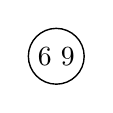
\begin{tikzpicture}
	\Vertex			{6 9}
\end{tikzpicture}

			\caption{Step 2}
		\end{minipage}\hfill
		\begin{minipage}{.25\textwidth}
			\centering
			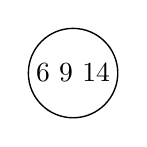
\begin{tikzpicture}
	\Vertex				{6 9 14}
\end{tikzpicture}
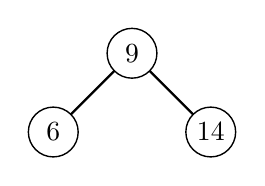
\begin{tikzpicture}
	\Vertex				{9}
	\Vertex[x=-1,y=-1]	{6}
	\Vertex[x=1,y=-1]	{14}
	
	\Edge				(9)(6)
	\Edge				(9)(14)
\end{tikzpicture}

			\caption{Step 3}
		\end{minipage}\hfill
	\end{figure}
	\begin{figure}[H]
		\centering
		\begin{minipage}{.33\textwidth}
			\centering
			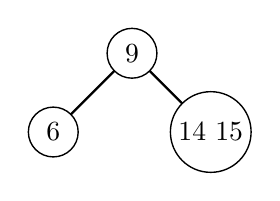
\begin{tikzpicture}
	\Vertex				{9}
	\Vertex[x=-1,y=-1]	{6}
	\Vertex[x=1,y=-1]	{14 15}
	
	\Edge				(9)(6)
	\Edge				(9)(14 15)
\end{tikzpicture}

			\caption{Step 4}
		\end{minipage}\hfill
		\begin{minipage}{.33\textwidth}
			\centering
			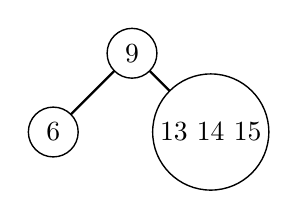
\begin{tikzpicture}
	\Vertex				{9}
	\Vertex[x=-1,y=-1]	{6}
	\Vertex[x=1,y=-1]	{13 14 15}
	
	\Edge				(9)(6)
	\Edge				(9)(13 14 15)
\end{tikzpicture}
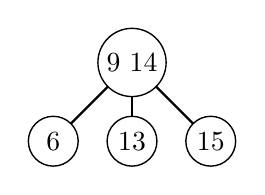
\begin{tikzpicture}
	\Vertex				{9 14}
	\Vertex[x=-1,y=-1]	{6}
	\Vertex[x=0,y=-1]	{13}
	\Vertex[x=1,y=-1]	{15}
	
	\Edge				(9 14)(6)
	\Edge				(9 14)(13)
	\Edge				(9 14)(15)
\end{tikzpicture}

			\caption{Step 5}
		\end{minipage}\hfill
		\begin{minipage}{.33\textwidth}
			\centering
			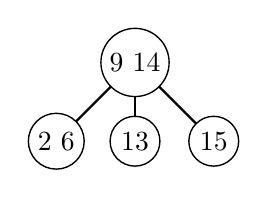
\begin{tikzpicture}
	\Vertex				{9 14}
	\Vertex[x=-1,y=-1]	{2 6}
	\Vertex[x=0,y=-1]	{13}
	\Vertex[x=1,y=-1]	{15}
	
	\Edge				(9 14)(2 6)
	\Edge				(9 14)(13)
	\Edge				(9 14)(15)
\end{tikzpicture}

			\caption{Step 6}
		\end{minipage}\hfill
	\end{figure}
	\begin{figure}[H]
		\centering
		\begin{minipage}{.33\textwidth}
			\centering
			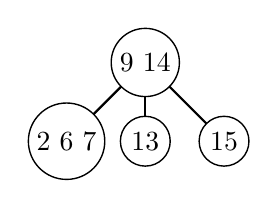
\begin{tikzpicture}
	\Vertex				{9 14}
	\Vertex[x=-1,y=-1]	{2 6 7}
	\Vertex[x=0,y=-1]	{13}
	\Vertex[x=1,y=-1]	{15}
	
	\Edge				(9 14)(2 6 7)
	\Edge				(9 14)(13)
	\Edge				(9 14)(15)
\end{tikzpicture}
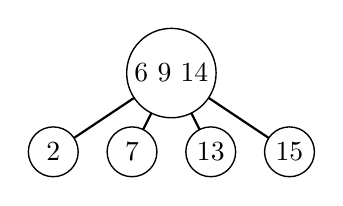
\begin{tikzpicture}
	\Vertex					{6 9 14}
	\Vertex[x=-1.5,y=-1]	{2}
	\Vertex[x=-0.5,y=-1]	{7}
	\Vertex[x=0.5,y=-1]		{13}
	\Vertex[x=1.5,y=-1]		{15}
	
	\Edge				(6 9 14)(2)
	\Edge				(6 9 14)(7)
	\Edge				(6 9 14)(13)
	\Edge				(6 9 14)(15)
\end{tikzpicture}
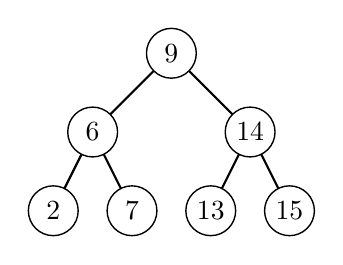
\begin{tikzpicture}
	\Vertex					{9}
	\Vertex[x=-1,y=-1]		{6}
	\Vertex[x=1,y=-1]		{14}
	\Vertex[x=-1.5,y=-2]	{2}
	\Vertex[x=-0.5,y=-2]	{7}
	\Vertex[x=0.5,y=-2]		{13}
	\Vertex[x=1.5,y=-2]		{15}
	
	\Edge			(9)(6)
	\Edge			(9)(14)
	\Edge			(6)(2)
	\Edge			(6)(7)
	\Edge			(14)(13)
	\Edge			(14)(15)
\end{tikzpicture}

			\caption{Step 7}
		\end{minipage}\hfill
		\begin{minipage}{.33\textwidth}
			\centering
			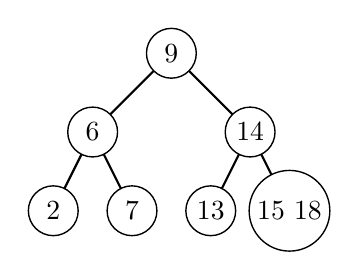
\begin{tikzpicture}
	\Vertex					{9}
	\Vertex[x=-1,y=-1]		{6}
	\Vertex[x=1,y=-1]		{14}
	\Vertex[x=-1.5,y=-2]	{2}
	\Vertex[x=-0.5,y=-2]	{7}
	\Vertex[x=0.5,y=-2]		{13}
	\Vertex[x=1.5,y=-2]		{15 18}
	
	\Edge			(9)(6)
	\Edge			(9)(14)
	\Edge			(6)(2)
	\Edge			(6)(7)
	\Edge			(14)(13)
	\Edge			(14)(15 18)
\end{tikzpicture}

			\caption{Step 8}
		\end{minipage}\hfill
		\begin{minipage}{.33\textwidth}
			\centering
			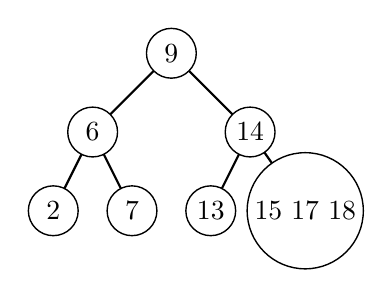
\begin{tikzpicture}
	\Vertex					{9}
	\Vertex[x=-1,y=-1]		{6}
	\Vertex[x=1,y=-1]		{14}
	\Vertex[x=-1.5,y=-2]	{2}
	\Vertex[x=-0.5,y=-2]	{7}
	\Vertex[x=0.5,y=-2]		{13}
	\Vertex[x=1.7,y=-2]		{15 17 18}
	
	\Edge			(9)(6)
	\Edge			(9)(14)
	\Edge			(6)(2)
	\Edge			(6)(7)
	\Edge			(14)(13)
	\Edge			(14)(15 17 18)
\end{tikzpicture}
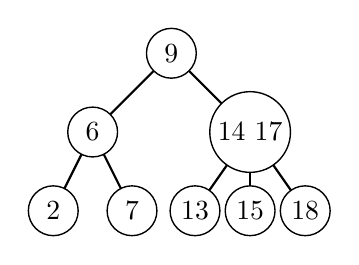
\begin{tikzpicture}
	\Vertex					{9}
	\Vertex[x=-1,y=-1]		{6}
	\Vertex[x=1,y=-1]		{14 17}
	\Vertex[x=-1.5,y=-2]	{2}
	\Vertex[x=-0.5,y=-2]	{7}
	\Vertex[x=0.3,y=-2]		{13}
	\Vertex[x=1,y=-2]		{15}
	\Vertex[x=1.7,y=-2]		{18}
	
	\Edge			(9)(6)
	\Edge			(9)(14 17)
	\Edge			(6)(2)
	\Edge			(6)(7)
	\Edge			(14 17)(13)
	\Edge			(14 17)(15)
	\Edge			(14 17)(18)
\end{tikzpicture}

			\caption{Step 9}
		\end{minipage}\hfill
	\end{figure}
\section{Relaxed AVL trees}
	First, we define $N(h)$ as a recurrence relation and prove its validity.\\
	Claim: \[N(h) =
				\begin{cases}
					1 & h=0\\
					2 & h=1\\
					3 & h=2\\
					N(h-1)+N(h-3)+1 & h > 2
				\end{cases}
			\]
	Proof: (Induction)\\
	$N(h)$ is defined as the minimum number of vertices in a Relaxed AVL tree. It is clear to see
	from this definition that the the three base cases hold.\\
	Suppose the claim holds for all $l<h$.\\
	We will now show that the claim also holds for $h$ by constructing the Relaxed AVL tree of height $h$ with the minimum number of vertices.
	Take one vertex and let it be the root of our new tree. Our tree must have height $h$, so at least one of its children must have height $h-1$.
	By our hypothesis, $N(h-1)$ is the minimum number of vertices in a Relaxed AVL tree of height $h-1$. In order to satisfy the Relaxed height-balance
	property, our tree's children's heights must not differ by more than two, so to minimize our vertices we shall choose our next child to have height $n-3$.
	Again, by our hypothesis we know that the minimum number of vertices in a Relaxed AVL tree of height $h-3$ is $N(h-3)$. If we now consider our tree
	with one root vertex and two children, both of which are also Relaxed AVL trees with $N(h-1)$ and $N(h-2)$ vertices, our number of vertices will be
	$N(h-1)+N(h-3)+1$. Thus our definition of $N(h)$ holds for all $h$.
	\newline
	\newline
	We will now show that $N(h)\in{\Omega{(k^h)}}$ for some $k>1$.\\
	It is sufficient to show that $N(h)\ge{ck^h}$ for some $c>0,k>1$.
	Claim: There exists some $c>0,k>1$ such that $N(h)\ge{ck^h}$ for all $h$.\\
	Proof: (Induction)
	\begin{align*}
		N(0)=1: \quad& 1\ge{ck^0}\quad\text{if}\quad\frac{1}{k^0}\ge{c}\\[1em]
		N(1)=2: \quad& 2\ge{ck^1}\quad\text{if}\quad\frac{1}{k^1}\ge{c}\\[1em]
		N(2)=3: \quad& 3\ge{ck^2}\quad\text{if}\quad\frac{1}{k^2}\ge{c}
	\end{align*}
	Note that the cases for $h=0$ and $h=1$ also hold when $c\le\frac{1}{k^2}$, so let $c\le\frac{1}{k^2}$.\\
	Suppose $N(l)\ge{ck^l}$ for all $l<h$.\\
	We want to show that $N(h)\ge{ck^h}$ for some $c>0,k>1$. Recall the definition for $N(h)$:
	\[N(h)=N(h-1)+N(h-3)+1\]
	By our hypothesis, we have
	\begin{align*}
		N(h)&\ge{ck^{h-1}+ck^{h-3}+1}\\
		&\ge{ck^{h-1}+ck^{h-3}}
	\end{align*}
	So if we can show that $ck^{h-1}+ck^{h-3}\ge{ck^h}$, it would be sufficient to show that $N(h)\ge{ck^h}$.
	\begin{align*}
		&ck^{h-1}+ck^{h-3}\ge{ck^h}\\
		&\implies{\frac{ck^{h-1}+ck^{h-3}}{ck^{h-3}}\ge{\frac{ck^h}{ck^{h-3}}}}\\
		&\implies{k^2+1\ge{k^3}}\\
		&\implies{k^3-k^2-1\le{0}}
	\end{align*}
	The real root of the polynomial $k^3-k^2-1=0$ is approximately $1.4655$, so any value for $k$ less than this
	value will do. Recall that we defined $c\le\frac{1}{k^2}$. So the claim holds for $k=1.4655$ and $c=\frac{1}{1.4655^2}$,
	and therefore $N(h)\ge{\frac{1}{1.4655^2}1.4655^{h}}$ for any value of $h$.\\
	Thus we have proven the claim that $N(h)\ge{ck^h}$ for some $c>0,k>1$, and therefore $N(h)\in\Omega{(1.4655^h)}$.

\end{document}
